\begin{figure}[h]
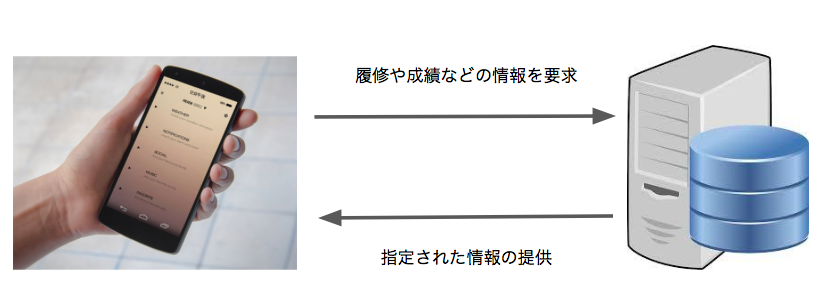
\includegraphics[scale = 0.5]{./nagare.png}
\caption{情報の流れ}
\label{flow}
\end{figure}

システムとしては、まず大学PCで使用されているユーザ名とパスワードを用いて認証を行い、ログインしてもらいます。その後、図\ref{flow}の様に端末側からの履修状況や成績等の情報要求に対して、サーバ側では指定された情報提供を行う事で履修状況の閲覧が可能なアプリケーションとなっています。また、Web上で履修を変更した場合にも、即時反映できるようになっています。
